\chapter{Partidas-Exemplo}\label{chap:cinco}

\section{Partida-Exemplo em um Tabuleiro \texorpdfstring{6$\times$6}{6x6}}

A partida a seguir ilustra jogadas perfeitas em um tabuleiro 6$\times$6, o menor tamanho em que Go é interessante de ser jogado.

\emph{Dia.\@~1}. Isso pode ser chamado de abertura. Preto começa por tentar controlar o lado direito com 1 e 3; e Branco, o lado esquerdo com 2 e 4. Preto se dobra em volta de Branco com 5 e 7, e Branco resiste com 6 e 8.

\begin{figure}[h!]
  \centering
  \begin{subfigure}[t]{.3\textwidth}
    \centering
    
\includegraphics[width=1\textwidth]{5 - Dia 1}
    \captionsetup{justification=centering}
    \caption*{\emph{Dia.\@~1. (1-8)}}
  \end{subfigure}
  \hfill
  \begin{subfigure}[t]{.3\textwidth}
    \centering
    
\includegraphics[width=1\textwidth]{5 - Dia 2}
    \captionsetup{justification=centering}
    \caption*{\emph{Dia.\@~2. (9)}}
  \end{subfigure}
  \hfill
  \begin{subfigure}[t]{.3\textwidth}
    \centering
    
\includegraphics[width=1\textwidth]{5 - Dia 3}
    \captionsetup{justification=centering}
    \caption*{\emph{Dia.\@~3. (10-11)}}
  \end{subfigure}
\end{figure}

\emph{Dia.\@~2}. Preto pressiona sua vantagem através do corte em 9. Isso põe as duas pedras marcadas em atari --- as pedras pretas estão ocupando todas as liberdades brancas exceto uma. Note que as pedras brancas marcadas não estão diretamente conectadas às outras pedras brancas.

\emph{Dia.\@~3}. Branco resgata suas duas pedras pela conexão com 10, e a pedra preta marcada agora está em atari. Preto ignora isso e joga 11, colocando a pedra branca em atari.

\pagebreak

\emph{Dia.\@~4}. Branco escapa do atari descendo para 12. Preto conecta com 13 para prevenir que Branco o corte ali. A pedra preta marcada ainda está sob atari. Entretanto, ela não pode escapar, então Branco não se apressa em capturá-la e corta em 14, colocando outra pedra preta em atari.

\begin{figure}[h!]
  \centering
  \begin{subfigure}[t]{.3\textwidth}
    \centering
    
\includegraphics[width=1\textwidth]{5 - Dia 4}
    \captionsetup{justification=centering}
    \caption*{\emph{Dia.\@~4. (12-14)}}
  \end{subfigure}
  \hfill
  \begin{subfigure}[t]{.3\textwidth}
    \centering
    
\includegraphics[width=1\textwidth]{5 - Dia 5}
    \captionsetup{justification=centering}
    \caption*{\emph{Dia.\@~5. (15-18)}}
  \end{subfigure}
  \hfill
  \begin{subfigure}[t]{.3\textwidth}
    \centering
    
\includegraphics[width=1\textwidth]{5 - Dia 6}
    \captionsetup{justification=centering}
    \caption*{\emph{Dia.\@~6. (19-21)}}
  \end{subfigure}
\end{figure}

\emph{Dia.\@~5}. Preto joga um atari com 15 e Branco captura com 16, tomando um prisioneiro. Preto agora desce para 17, ameaçando jogar em 18 e desprivilegiar Branco de um ponto. Sendo assim, Branco precisa conectar em 18. Esse é o último movimento da partida, valendo um ponto.

\emph{Dia.\@~6}. Preto conecta com 19, preparando para tomar o último ponto neutro em 21. Branco não pode jogar em 21, então ele captura com 20, tomando outro prisioneiro.

\pagebreak

\emph{Dia.\@~7}. Após Preto 21 no \emph{Dia.\@~6}, não há mais pontos a serem ganhos ou disputados, então Branco passa. Preto também passa. De acordo com a \emph{Regra 8}, o jogo termina.

\begin{figure}[h!]
  \centering
  \begin{subfigure}[t]{.3\textwidth}
    \centering
    
\includegraphics[width=1\textwidth]{5 - Dia 7}
    \captionsetup{justification=raggedright,singlelinecheck=false,margin={.20in,.05in}}
    \caption*{\emph{Dia.\@~7. Partida finalizada}}
  \end{subfigure}
  \hspace{1cm}
  \begin{subfigure}[t]{.3\textwidth}
    \centering
    
\includegraphics[width=1\textwidth]{5 - Dia 8}
    \captionsetup{justification=centering}
    \caption*{\emph{Dia.\@~8}}
  \end{subfigure}
\end{figure}

\emph{Dia.\@~8}. Branco possui dois prisioneiros, então ele os coloca no território preto --- as duas pedras marcadas. Os territórios são agora contados. Branco possui 6 pontos, e Preto, 9.

\textbf{Preto vence por 3 pontos.}

\pagebreak

\section{Perguntas e Respostas}\label{section:5.2:seki}

\begin{itemize}
  \item[\textbf{Pergunta}]
    Ao invés de 19 no \emph{Dia.\@~6}, será que Preto não poderia jogar atari em 21?
  \item[\textbf{Resposta}]
    Se Preto fizer atari imediatamente com 1 no \emph{Dia.\@~9}, ele se coloca em atari e perde duas pedras após a captura Branca com 2.

    \begin{figure}[h!]
      \centering
      \begin{subfigure}[t]{.3\textwidth}
        \centering
        
\includegraphics[width=.9\textwidth]{5 - Dia 9}
        \captionsetup{justification=centering}
        \caption*{\emph{Dia.\@~9}}
      \end{subfigure}
      \hspace{1cm}
      \begin{subfigure}[t]{.3\textwidth}
        \centering
        
\includegraphics[width=.9\textwidth]{5 - Dia 10}
        \captionsetup{justification=centering}
        \caption*{\emph{Dia.\@~10}}
      \end{subfigure}
    \end{figure}

  \item[\textbf{Pergunta}]
    Ao invés de capturar com 20 no \emph{Dia.\@~6}, será que Branco não poderia jogar no último ponto neutro em 21?
  \item[\textbf{Resposta}]
    Se Branco jogar imediatamente em 1 no \emph{Dia.\@~10}, ele coloca três de suas pedras em atari, e Preto procederia com a captura em 2.
  \item[\textbf{Pergunta}]
    Por que Branco passou no \emph{Dia.\@~7}? Por que ele não tenta invadir o território com 1 no \emph{Dia.\@~11}?

  \item[\textbf{Resposta}]
    Não há regra que previna Branco de invadir. Mas ele percebe que isso seria de nenhuma utilidade. Preto responderia com 2 no \emph{Dia.\@~12}, colocando a pedra invasora em atari, e, quando Preto captura com 6, Branco perderia sua força invasora completamente.

    \begin{figure}[h!]
      \centering
      \begin{subfigure}[t]{.3\textwidth}
        \centering
        
\includegraphics[width=.9\textwidth]{5 - Dia 11}
        \captionsetup{justification=centering}
        \caption*{\emph{Dia.\@~11}}
      \end{subfigure}
      \hspace{1cm}
      \begin{subfigure}[t]{.3\textwidth}
        \centering
        
\includegraphics[width=.9\textwidth]{5 - Dia 12}
        \captionsetup{justification=centering}
        \caption*{\emph{Dia.\@~12}}
      \end{subfigure}
    \end{figure}

  \item[\textbf{Pergunta}]
    Se Branco continuar insistindo na invasão, será que ele não conseguirá, no final, ocupar todos os pontos dentro do grupo Preto e, assim, capturá-lo?

    \begin{figure}[h!]
      \centering
      \begin{subfigure}[t]{.3\textwidth}
        \centering
        
\includegraphics[width=.9\textwidth]{5 - Dia 13}
        \captionsetup{justification=centering}
        \caption*{\emph{Dia.\@~13}}
      \end{subfigure}
      \hfill
      \begin{subfigure}[t]{.3\textwidth}
        \centering
        
\includegraphics[width=.9\textwidth]{5 - Dia 14}
        \captionsetup{justification=centering}
        \caption*{\emph{Dia.\@~14}}
      \end{subfigure}
      \hfill
      \begin{subfigure}[t]{.3\textwidth}
        \centering
        
\includegraphics[width=.9\textwidth]{5 - Dia 15}
        \captionsetup{justification=centering}
        \caption*{\emph{Dia.\@~15}}
      \end{subfigure}
    \end{figure}

  \item[\textbf{Resposta}]
    Ele é bem-vindo a tentar, como no \emph{Dia.\@~13}, mas ele não será bem-sucedido. Após Branco 7 e 9, Preto esmaga aquelas duas pedras com 10 --- Branco não pode conectar no ponto 1-1, já que seria suicídio, um movimento ilegal. Branco põe o grupo preto de onze pedras em atari com 11 no \emph{Dia.\@~14} e Preto captura duas pedras com 14. No final, Branco esgota os possíveis pontos de invasão. A posição agora aparenta ser \emph{Dia.\@~15} e Preto ainda vence por 3 pontos. Lembre-se que as pedras brancas voltarão para o território Branco quando a partida for contabilizada. Branco pode tentar novamente em \textbf{A}, mas Preto capturará imediatamente com \textbf{B}, e vice-versa.

    O que faz com que o grupo preto inteiro no \emph{Dia.\@~15} seja invulnerável à captura são os vários buracos, ou olhos, que ele possui. Branco pode jogar somente uma pedra por vez, portanto ele jamais conseguirá preencher todos esses olhos simultaneamente, sem se suicidar, como ele deveria, para capturar o grupo preto.

  \pagebreak

  \item[\textbf{Pergunta}]
    Quantos ``buracos''  ou ``olhos''  são necessários para que um grupo esteja seguro?
  \item[\textbf{Resposta}]
    Ele precisa de dois, pelo menos. \emph{Dia.\@~16} mostra dois exemplos. Os dois grupos pretos estão vivos com dois olhos cada um. Na verdade, Branco não possui um movimento legal para atacar também. Branco, com seus dois grandes espaços de olhos, também está vivo. Preto pode jogar dentro do grupo branco, mas Branco pode facilmente capturar os invasores.

    \begin{figure}[h!]
      \centering
      \begin{subfigure}[t]{.3\textwidth}
        \centering
        
\includegraphics[width=.9\textwidth]{5 - Dia 16}
        \captionsetup{justification=centering}
        \caption*{\emph{Dia.\@~16}}
      \end{subfigure}
      \hfill
      \begin{subfigure}[t]{.3\textwidth}
        \centering
        
\includegraphics[width=.9\textwidth]{5 - Dia 17}
        \captionsetup{justification=centering}
        \caption*{\emph{Dia.\@~17}}
      \end{subfigure}
      \hfill
      \begin{subfigure}[t]{.3\textwidth}
        \centering
        
\includegraphics[width=.9\textwidth]{5 - Dia 18}
        \caption*{\emph{Dia.\@~18. Branco 3 em 1}}
      \end{subfigure}
    \end{figure}

    Você deveria também notar que os olhos precisam estar separados. O grupo preto no canto inferior esquerdo do \emph{Dia.\@~17} não está vivo, mas morto. Ele não consegue evitar de ser capturado. Talvez possa parecer que ele possui dois olhos, mas estes, neste caso, não são separáveis ou distintos. Branco 1 no \emph{Dia.\@~18} coloca Preto em atari. Preto pode capturar com 2, mas Branco só joga novamente 3 em 1, privando o grupo preto de sua última liberdade e, assim, capturando todas as cinco pedras pretas.

    Outra coisa sobre a qual se atentar é olho falso, como o que o grupo preto possui no canto superior direito do \emph{Dia.\@~18} em \textbf{A}. Esse grupo também está morto. Branco \textbf{A} captura as três pedras marcadas e põe as outras duas pedras sob atari.

  \pagebreak

  \item[\textbf{Pergunta}]
    Um grupo sempre precisa estar apto a criar dois olhos para estar vivo?

    \begin{figure}[h!]
      \centering
      \begin{subfigure}[t]{.4\textwidth}
        \centering
        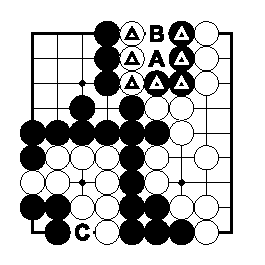
\includegraphics[width=1\textwidth]{5 - Dia 19}
        \captionsetup{justification=centering}
        \caption*{\emph{Dia.\@~19}}
      \end{subfigure}
    \end{figure}
  \item[\textbf{Resposta}]
    Geralmente, mas há exceções. No \emph{Dia.\@~19}, o grupo preto marcado e o grupo branco não possuem nenhum olho, mas ambos compartilham liberdades. Nenhum dos lados pode atacar o outro jogando \textbf{A} ou \textbf{B} sem se colocar em atari, então nenhum dos lados deveria jogar nessa região, ou seja, ambos os grupos estão vivos. Este tipo de impasse local é chamado de \emph{seki}. Os pontos vazios entre as pedras marcadas não contam como território para nenhum dos lados.

    Há outro seki no canto inferior esquerdo do \emph{Dia.\@~19}. O grupo preto de três pedras e o grupo branco cercando-o ambos possuem um olho só, e nenhum deles pode ocupar o ponto \textbf{C} entre eles sem se colocar em atari. (O ponto \textbf{C} também não é território.)
\end{itemize}

\pagebreak

\section{Partida-Exemplo em um Tabuleiro \texorpdfstring{9$\times$9}{9x9}}

\emph{Dia.\@~1}. A boa estratégia dita que movimentos de abertura sejam feitos na terceira linha ou acima, em relação às bordas do tabuleiro. Neste caso, no entanto, Preto 1 e Branco 2 são jogados nas quartas linhas, um dos motivos sendo as peculiaridades do tabuleiro 9$\times$9.

\begin{figure}[h!]
  \centering
  \begin{subfigure}[t]{.3\textwidth}
    \centering
    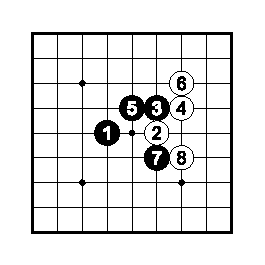
\includegraphics[width=1.05\textwidth]{5 - Exemplo - Dia 1}
    \captionsetup{justification=centering}
    \caption*{\emph{Dia.\@~1. (1-8)}}
  \end{subfigure}
  \hfill
  \begin{subfigure}[t]{.3\textwidth}
    \centering
    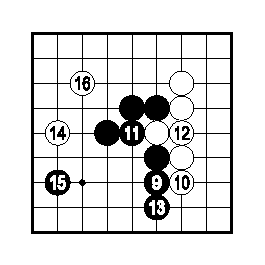
\includegraphics[width=1.05\textwidth]{5 - Exemplo - Dia 2}
    \captionsetup{justification=centering}
    \caption*{\emph{Dia.\@~2. (9-16)}}
  \end{subfigure}
  \hfill
  \begin{subfigure}[t]{.3\textwidth}
    \centering
    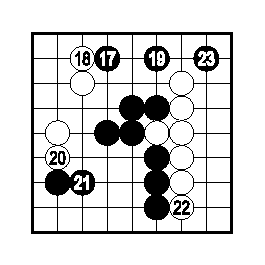
\includegraphics[width=1.05\textwidth]{5 - Exemplo - Dia 3}
    \captionsetup{justification=centering}
    \caption*{\emph{Dia.\@~3. (17-23)}}
  \end{subfigure}
\end{figure}

\emph{Dia.\@~2}. Preto 11 faz atari na pedra branca, então Branco conecta em 12. Tendo construído um grupo vivo à direita, Branco invade o lado esquerdo com 14 e inicia o estabelecimento de outro grupo vivo à esquerda com 16.

\emph{Dia.\@~3}. Branco defende seu grupo no lado esquerdo com 18 e 20, e, então, seu grupo à direita com 22. Preto pula para o lado direito com 23 e o fim de jogo se inicia. Pulos de um espaço como 19 e 23 são frequentemente boas jogadas.

\pagebreak

\emph{Dia.\@~4}. Branco detém a intrusão preta ao lado esquerdo com 24 e 26. As jogadas começam, a partir de agora, a focar nas bordas do tabuleiro.

\begin{figure}[h!]
  \centering
  \begin{subfigure}[t]{.3\textwidth}
    \centering
    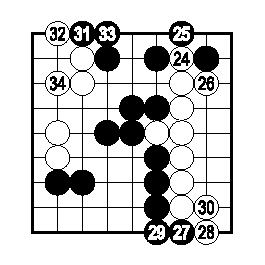
\includegraphics[width=1.05\textwidth]{5 - Exemplo - Dia 4}
    \captionsetup{justification=centering}
    \caption*{\emph{Dia.\@~4. (24-34)}}
  \end{subfigure}
  \hspace{1cm}
  \begin{subfigure}[t]{.3\textwidth}
    \centering
    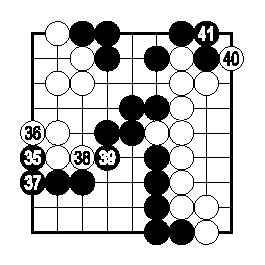
\includegraphics[width=1.05\textwidth]{5 - Exemplo - Dia 5}
    \captionsetup{justification=centering}
    \caption*{\emph{Dia.\@~5. (35-41)}}
  \end{subfigure}
\end{figure}

\emph{Dia.\@~5}. O fim de jogo continua com Preto 35 até o atari de Branco 40.

\emph{Dia.\@~6}. Branco 50 é um sacrifício que, mais tarde, forçará Preto a conectar em 55. No final da partida, Branco perdeu um prisioneiro --- a pedra em 50 --- e Preto 53 é uma pedra morta.

\begin{figure}[h!]
  \centering
  \begin{subfigure}[t]{.3\textwidth}
    \centering
    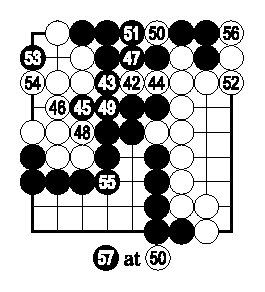
\includegraphics[width=1.05\textwidth]{5 - Exemplo - Dia 6}
    \captionsetup{justification=centering}
    \caption*{\emph{Dia.\@~6. (42-57)}}
  \end{subfigure}
  \hfill
  \begin{subfigure}[t]{.3\textwidth}
    \centering
    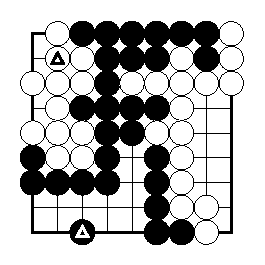
\includegraphics[width=1.05\textwidth]{5 - Exemplo - Dia 7}
    \captionsetup{justification=centering}
    \caption*{\emph{Dia.\@~7. Prisioneiros}}
  \end{subfigure}
  \hfill
  \begin{subfigure}[t]{.3\textwidth}
    \centering
    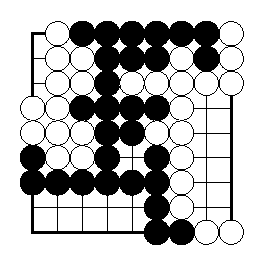
\includegraphics[width=1.05\textwidth]{5 - Exemplo - Dia 8}
    \captionsetup{justification=centering}
    \caption*{\emph{Dia.\@~8. Rearranjo}}
  \end{subfigure}
\end{figure}

\emph{Dia.\@~7}. O prisioneiro branco é substituído dentro do território branco, e a pedra preta morta --- 53 no \emph{Dia.\@~6} --- é removida e preenche o interior do território preto. Essas pedras são indicadas pelas pedras marcadas.

\emph{Dia.\@~8}. É costumeiro rearranjar os territórios durante a contagem, para torná-lo mais facilmente reconhecível em termos de múltiplos de 5 ou de 10. Nesta partida, Preto possui 11 pontos de território, e Branco, 13, portanto, Branco vence por dois pontos.